% Name: Trapezoidal rule
% Description: Four trapezoids whose slanted tops join points on the curve, approximating the integral from a to b, with the rule's formula below.
% Tags: trapezoidal rule, numerical integration, approximation, integral

\usetikzlibrary{arrows.meta}

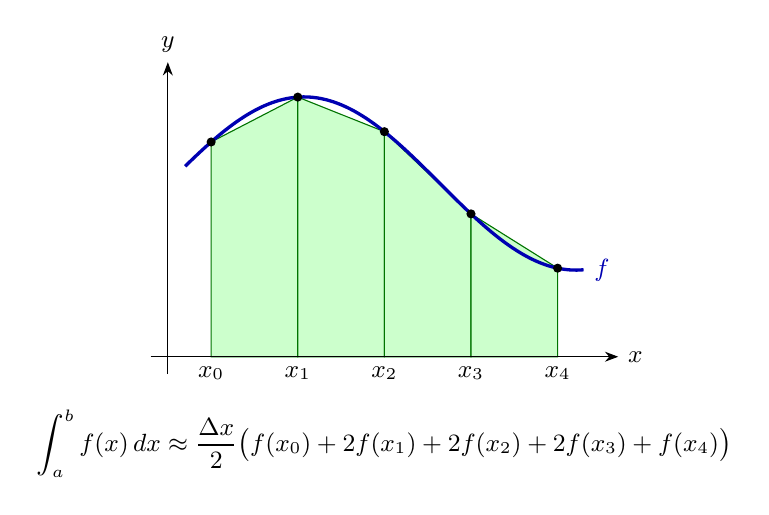
\begin{tikzpicture}[>={Stealth}, scale=1.1, every node/.style={font=\small}]
  \foreach \i in {0,...,3} {
    \pgfmathsetmacro\x{0.5 + \i}
    \draw[fill=green!20, draw=green!45!black] (\x,0) -- (\x,{2 + sin(deg(\x))}) -- (\x+1,{2 + sin(deg(\x+1))}) -- (\x+1,0) -- cycle;
  }
  \draw[->] (-0.2,0) -- (5.2,0) node[right] {$x$};
  \draw[->] (0,-0.2) -- (0,3.4) node[above] {$y$};
  \draw[very thick, blue!70!black, domain=0.2:4.8, samples=60, smooth] plot (\x, {2 + sin(deg(\x))}) node[right] {$f$};
  \foreach \i in {0,...,4} {
    \pgfmathsetmacro\x{0.5 + \i}
    \fill (\x,{2 + sin(deg(\x))}) circle (1.5pt);
    \node[below] at (\x,0) {$x_\i$};
  }
  \node at (2.5,-1) {$\displaystyle\int_a^b f(x)\,dx \approx \frac{\Delta x}{2}\bigl(f(x_0) + 2f(x_1) + 2f(x_2) + 2f(x_3) + f(x_4)\bigr)$};
\end{tikzpicture}
